\documentclass[usenames,dvipsnames, 9pt,aspectratio=169]{beamer}
\usepackage{amsmath,amsfonts,amssymb}
\usepackage{mathtools}
\usepackage{etex} %for Windows
\usepackage[utf8]{inputenc}
\usepackage[english]{babel} 
%\usepackage[russian]{babel}
%\usepackage{microtype}			% Better interword spacing and additional kerning.
\usepackage{ellipsis}			% Adjusted space with \dots between two words.
\usepackage{graphicx}
\usepackage{pstricks}

\usepackage{xcolor}


\usepackage{changepage}

\usepackage{algorithm}
\usepackage{algpseudocode}
%\usepackage[]{algorithm2e}
%\usepackage{algorithmic}

%\usepackage{tcolorbox}



\addtobeamertemplate{footline}{%
	\setlength\unitlength{1ex}%
	\begin{picture}(0,0) 
	% \put{} defines the position of the frame
	\put(155,2){\makebox(0,0)[bl]{
			\includegraphics[scale=0.15]{avatar_colour}
	}}%
	\end{picture}%
}{}


\usepackage{tikz}
\usetikzlibrary{tikzmark,calc}
\usetikzlibrary{positioning, backgrounds}
\usetikzlibrary{arrows, chains, matrix, scopes, patterns, shapes, fit}
\usetikzlibrary{mindmap,trees,shadows}
\usetikzlibrary{decorations.pathreplacing}

\usepackage{pgfplots}

\pgfmathdeclarefunction{gauss}{2}{%
	\pgfmathparse{1/(#2*sqrt(2*pi))*exp(-((x-#1)^2)/(2*#2^2))}%
}


\tikzset{
	invisible/.style={opacity=0},
	visible on/.style={alt={#1{}{invisible}}},
	alt/.code args={<#1>#2#3}{%
		\alt<#1>{\pgfkeysalso{#2}}{\pgfkeysalso{#3}} % \pgfkeysalso doesn't change the path
	},
}

\newcommand\strikeout[2][]{%
	\begin{tabular}[b]{@{}c@{}} 
		\makebox(0,0)[cb]{{#1}} \\[-0.2\normalbaselineskip]
		\rlap{\color{Orange}\rule[0.5ex]{\widthof{#2}}{1.5pt}}#2
\end{tabular}}

\newcommand\Fontvi{\fontsize{11}{13.2}\selectfont}

\usepackage{listings} % for C++ code

\usepackage{braket}
%\usepackage[braket, qm]{qcircuit}



\usepackage[T1]{fontenc}
%\usepackage[sfdefault,scaled=.85]{FiraSans}
%\usepackage{newtxsf}
%\usepackage[nomap]{FiraMono}





\usefonttheme[onlymath]{serif}
\renewcommand\sfdefault{cmbr}

\renewcommand{\bfdefault}{sb}

\definecolor{CharCoalDark}{RGB}{13, 16, 19}
\definecolor{Orange}{RGB}{255, 165,0}
\definecolor{DarkOrange}{RGB}{255, 165,0}
\definecolor{LightSalmon}{RGB}{255, 160, 122}
\definecolor{LeafGreen}{RGB}{34, 139,  34}
\definecolor{Coral}{RGB}{255, 127, 80}
\definecolor{DarkTurquoise}{RGB}{0, 206, 209}

%\newtheorem{defRus}{Определение}
%\newtheorem{thmRus}{Теорема}
%s\newtheorem{corRus}{Следствие}


\setbeamercolor{background canvas}{bg=CharCoalDark}

\setbeamerfont{title}{series=\bfseries}
\setbeamercolor{title}{fg=Orange}
\setbeamercolor{section in toc}{fg=white}
\setbeamercolor{frametitle}{fg=Orange}
\setbeamercolor{normal text}{fg=white}
%\setbeamercolor{normal text}{fontsize=12pt}
\setbeamercolor{itemize item}{fg=Orange}
\setbeamercolor{itemize item item}{fg=Orange}
\setbeamercolor{enumerate item}{fg=Orange}
\setbeamercolor{block title}{bg=DarkOrange,fg=white}
\setbeamerfont{block title}{series=\bfseries}

\setbeamertemplate{itemize item}[circle]
%\setbeamertemplate{itemize subitem}[$\checkmark$]
\setbeamertemplate{itemize subitem}{\color{Orange}\Large$\textbullet$}
\setbeamertemplate{itemize subitem}{\color{Orange} \tiny $\blacksquare$}

% footnote without a marker
\newcommand\blfootnote[1]{%
	\begingroup
	\renewcommand\footnoterule{}
	\renewcommand\thefootnote{}\footnote{#1}%
	\addtocounter{footnote}{-1}%
	\endgroup
}

\newcommand*{\Scale}[2][4]{\scalebox{#1}{\ensuremath{#2}}}%

\newcommand\Item[1][]{%
	\ifx\relax#1\relax  \item \else \item[#1] \fi
	\abovedisplayskip=0pt\abovedisplayshortskip=0pt~\vspace*{-\baselineskip}}

\pgfdeclareradialshading{ring}{\pgfpoint{0cm}{0cm}}%
{rgb(0cm)=(1,1,1);
	rgb(0.7cm)=(1,1,1);
	rgb(0.719cm)=(1,1,1);
	rgb(0.72cm)=(0.975,0,0);
	rgb(0.9cm)=(1,1,1)}

\usepackage[absolute,overlay]{textpos} %to clip to a corner
\newcommand\FrameText[1]{%
	\begin{textblock*}{\paperwidth}(\textwidth-35pt, 10 pt)
		\raggedright #1\hspace{.5em}
\end{textblock*}}

\makeatletter
\let\save@measuring@true\measuring@true
\def\measuring@true{%
	\save@measuring@true
	\def\beamer@sortzero##1{\beamer@ifnextcharospec{\beamer@sortzeroread{##1}}{}}%
	\def\beamer@sortzeroread##1<##2>{}%
	\def\beamer@finalnospec{}%
}
\makeatother

\AtBeginSection[]
{
	\begin{frame}<beamer>
		\frametitle{Outline}
		\tableofcontents[currentsection]
	\end{frame}
}


%\institute{ENS Lyon}
\author{Elena Kirshanova \\ [10pt]
}
\titlegraphic{
	
	%\includegraphics[width=2.5cm]{erc_logo_gray}\hspace*{2.5cm}~%
	%\includegraphics[width=4.0cm]{ens_logo_gray}
}
\title{Perfect secrecy. One-time pad. PRGs.}

\date{ Course ``Information and Network Security'' \\ 	
	Lecture 2 \\ \today }


\setbeamertemplate{navigation symbols}{} %removes navigation

% proper highlightling of a code-snippet
\lstset{language=C++,
	keywordstyle=\color{magenta},
	stringstyle=\color{Goldenrod},
	commentstyle=\color{gray},
	breaklines=false,
	%morecomment=[l][\color{magenta}]{\#}
}

%\setlength{\parskip}{8pt}
\input{header} %all defs
\begin{document}
	
\begin{frame}
	\titlepage
\end{frame}


\begin{frame}{Some defs/conventions/notations}
\Large 
	\begin{block}{Polynomial time}
		An algorithm $\alg$ is called \emph{polynomial-time}, if for any input $n$, the runtime of $\alg$ is $\bigO(n^k)$ for any fixed $k$.
	\end{block}
\vspace{10pt}
Examples: 
\begin{itemize}
\LARGE
\item multiplying two $n$-bit numbers: $\bigO(n \log n)$ -- polynomial time
\item factoring an $n$-bit number: $\exp(\bigO(n^{1/3}\cdot (\log n)^{2/3})$ -- subexponential time
\end{itemize}
\vspace{10pt}
\Large
\pause
\begin{block}{Probabilistic Polynomial time}
	An algorithm $\alg$ is called \emph{probabilistic polynomial-time} (ppt), if it is polynomial time and uses randomness.
\end{block} 

\end{frame}


\begin{frame} {Some defs/conventions/notations}
\Large
	\begin{block}{Negligible function}
		A function $f: \N \rightarrow \R$ is called \emph{negligible} if for all  polynomials $p$ there exists $N \in \N$ so that for any $n \geq N$
		\[
			f(n) < \frac{1}{p(n)}.
		\]
	\end{block}

	\vspace{10pt}
	Examples: 
	\begin{itemize}
		\LARGE
		\item negligible functions: 
		\[
		\frac{1}{2^n}, \; \frac{1}{2^{\sqrt{n}}}, \;  \frac{1}{2^{\log^2(n)}}
		\]
		\item non-negligible functions: 
			\[
		\frac{1}{\log n}, \;  \frac{1}{n^2}, \;  \frac{1}{2^{\bigO(\log n)}} 
		\]
	\end{itemize}
\end{frame}

\begin{frame}{Basic principles of modern cryptography}
\large
	\begin{enumerate}
		\item \textbf{Kerckhoffs’ principle (1883)}:
		A cryptosystem should remain secure if everything about it, except the key, is publicly known.
		\item An adversary cannot derive any information about a plaintext from the corresponding ciphertext
		\item The attack model (i.e., what an adversary is allowed to do) must be clearly specified. \\
		Example: we restrict adversaries to be ppt algorithms
		\item The security assumption must as well be clearly specified. \\
	\end{enumerate}
	\pause
	\vspace{10pt}
	\centering
	 Security statement: \\
	\LARGE
	Under the assumption $X$, the construction $\Pi$ is secure in the $Y$ security model.
\end{frame}

\begin{frame}{Symmetric Encryption}
\Large
	Let $\lambda$ be a security parameter and $\mesS, \keyS, \cipS$ be resp.\ the plaintext, key, ciphertext spaces.
	A \emph{Symmetric Encryption Scheme} $\Pi = (\KeyGen, \Enc, \Dec )$ consists of three ppt algorithms: \\
	\begin{itemize}
		\item $\KeyGen(1^\lambda): k \leftarrow \keyS$ \\[10pt]
		\item $\Enc(k, m \in \mesS): c \leftarrow \Enc(k, m)$ \\[10pt]
		\item $\Dec{k, c \in \cipS}$ : $m' \leftarrow \Dec(k, c)$
	\end{itemize}
\pause
\vspace{20pt}
	The scheme $\Pi$ is called \emph{correct} if for all $k \in \keyS, m \in \mesS:$
	\[
		\Dec(k, \Enc(k, m)) == m.
	\]
\end{frame}

\begin{frame}{Perfect Secrecy}
\Large
	\begin{itemize}
		\item Let $\mesS, \keyS, \cipS$ be resp.\ the plaintext, key, ciphertext spaces
		
		\item Let $M \in \mesS$ be a random variable distributed according to a distribution defined over $\mesS$:
		$m$ is taken with  probability $\Pr[M = m]$.
		
		\item Analogously for $K \in \keyS, C \in \cipS$.
	\end{itemize}
\pause
	\begin{block}{Perfect secrecy}
		An encryption scheme $\Pi = (\KeyGen, \Enc, \Dec)$ is called \emph{perfectly secure} if for any distribution over $\mesS$
		\[
			\Pr \left[ M= m | C = c\right] = \Pr\left[M = m\right] \quad \forall m \in \mesS, c \in \cipS.
		\]
	\end{block}

	Equivalent definition:
	\[
		\Pr\left[\Enc(k, m_0) = c\right] = \Pr\left[\Enc(k, m_1) = c\right] \quad \forall m_0, m_1 \in \mesS, c \in \cipS.
	\]
\end{frame}

\begin{frame}{One-time pad (or Vernam cipher)}
\LARGE
\begin{block}{One-time pad}
	Let $\mesS, \keyS, \cipS = \{0,1\}^n$ s.t. $n = \lambda$.
	\begin{itemize}
		\item $\KeyGen(1^{\lambda}): k \leftarrow \{0,1\}^n$ \\[10pt]
		\item $\Enc(k, m \in \{0,1\}^n): c = k \oplus m$ \\[10pt]
		\item $\Dec(k, c \in \{0,1\}^n): m = k \oplus c$ \\[10pt]
	\end{itemize}
\end{block}

\begin{theorem}
	OTP is perfectly secure in the Ciphertext-only Attack (COA) model (i.e., an adversary sees only ciphertexts).
\end{theorem}

\end{frame}

\begin{frame}{Price to pay for perfect secrecy}
\Large
	\begin{block}{Size of $\keyS$}
		Let $\Pi$ be perfectly secure. Then
		\[
			|\keyS| \geq |\mesS|
		\]
	\end{block}

	\vspace{10pt}
	
	\begin{block}{Shannon's theorem}
		Let $\Pi = (\KeyGen, \Enc, \Dec)$ satisfy $|\keyS| = |\mesS| = |\cipS|$. Then $\Pi$ is perfectly secure iff
		\begin{enumerate}
			\item $\KeyGen$ chooses $k \leftarrow$ uniformly at random with prob.\ $\frac{1}{|\keyS|}$
			\item For all $m \in \mesS$, $c \in \cipS$, $\exists!$ $k \in \keyS:\,$ $c = \Enc(k,m)$.
		\end{enumerate}
	\end{block}
	
	\vspace{15pt}
	\large
	\centering
	See proofs in Katz\&Lindell \textit{Introduction to Modern Cryptography}
\end{frame}

\begin{frame}{Computational Security}
\Large
	{\color{Orange}\textbf{Perfect Secrecy}}
	\begin{itemize}
		\item Information-theoretic (strong) security against {\color{Orange}\textbf{unbounded}} adversary
		\item Impractical key space size
	\end{itemize}
		\vspace{15pt}
	{\color{Orange}\textbf{Computational Security}}
	\begin{itemize}
		\item We usually use keys of sizes $128, 256$ bits
		\item Security against {\color{Orange}\textbf{ppt}} adversaries
		\item Unbounded adversary with access to plaintext-ciphertext pairs $(m_i, c_i)$ can launch an exhaustive search for $k \in \keyS$ s.t.\ $\Enc(k, m_i) == c_i \; \forall i$.
	\end{itemize}
\end{frame}

\begin{frame}{Pseudorandom Generators (PRGs)}
\LARGE 
	Idea: `Stretch' truly random $\ell$-bits seed $s$ into a longer $L$-bits `random looking' string  
	\vspace{15pt}
	Define
	\LARGE
	\begin{align*}
		G : \{0,1\}^{\ell} & \rightarrow \{0,1\}^{L}:	\\
		s & \mapsto G(s) 
	\end{align*}
	
	{\color{Orange}\textbf{Intuition:}} an ppt adversary cannot tell the difference between $G(s)$ and $r \leftarrow \{0,1\}^L$.
	
\end{frame}

\begin{frame}{Statistical tests}
\Large 
A {\color{Orange}\textbf{Is $\Pi$ statistical test}} on $\{0,1\}^n$ is an algorithm $A$ s.t. $A(x)$ outputs $0$ (=``not random'') or $1$ (=``random'') \\[10pt]
\LARGE
\begin{enumerate}
	\item $A(x) = 1 \quad \abs{\# 0(x) - \# 1(x)} \leq 10 \sqrt{n}$  \\ [10pt]
	\item $A(x) = 1 \quad \abs{\# 00(x) - n/4} \leq 10 \sqrt{n}$  \\ [10pt]
	\item $A(x) = 1 \quad \max \mathsf{len}\{1...1(x) \} \leq 10 \log n$  \\ [10pt]
\end{enumerate}

\end{frame}

\begin{frame}{Secure PRG}
\Large
	\begin{block}{Formal definition}
	A PRG $G$ is an efficient deterministic algorithm that given a seed $s \in \mathcal{S} = \{0,1\}^{\ell}$ outputs an $r \in \mathcal{R} = \{0,1\}^L$ 
	
\end{block}
	{\color{Orange}\textbf{Attack game for PRG:}} \\
	\vspace{15pt}
	%For a given PRG $G$ and a given adversary $\mathcal{A}$, define 	{\color{Orange}\textbf{Experiment 0:}} and 	{\color{Orange}\textbf{Experiment 1:}}: \\
	{\color{Orange}\textbf{Experiment 0:}}
	The Challenger computes $r \in \mathcal{R}$ as
	\begin{align*}
		 \Huge	s &\leftarrow \mathcal{S} \\
		 \Huge	r & \leftarrow G(s)
	\end{align*}
	\pause
	{\color{Orange}\textbf{Experiment 1:}}
	The Challenger computes $r \in \mathcal{R}$ as
	\begin{align*}
		 \Huge	r & \leftarrow \{0,1\}^{L}
	\end{align*}
	Let $W_b$ be the event that $\mathcal{A}$ outputs $b$. \\
	 $\mathcal{A}$'s advantage: $	\mathsf{PRGadv} \left[  \mathcal{A}, G \right ] = |\Pr[W_0] - \Pr[W_1]|$. \\[5pt]
	 
	 A PRG $G$ is {\color{Orange}\textbf{secure}} if $	\mathsf{PRGadv}$ is negligible for all ppt $\mathcal{A}$.
	 

\end{frame}

\begin{frame}{Stream Cipher = OTP with keys output by a PRG}
\LARGE
	Let $G: \{0,1\}^{\ell} \rightarrow \{0,1\}^L$ \\[5pt]
	
	The {\color{Orange}\textbf{stream cipher}} $\Pi = (\KeyGen, \Enc, \Dec)$ is defined over
	\begin{itemize}
		\item $\keyS = \{0,1\}^{\ell}$ \\
		\item $\mesS = \{0,1\}^{L}$ \\
		\item $\cipS = \{0,1\}^{L}$ \\
	\end{itemize}
	\vspace{10pt}
	For $s \in \{0,1\}^{\ell}$
	\begin{itemize}
		\item $\Enc(s, m \in \{0,1\}^L): c = G(s) \oplus m$ \\[10pt]
		\item $\Dec(s, c \in \{0,1\}^L): m = G(s)\oplus c$ \\
	\end{itemize}

\end{frame}

\begin{frame}{Semantic Security}
		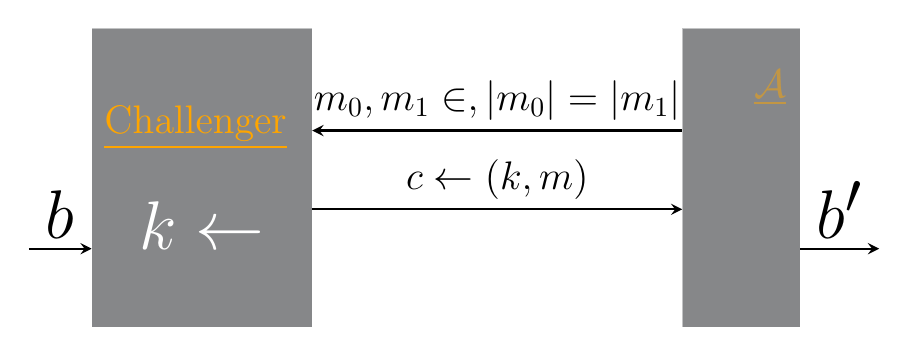
\begin{tikzpicture}
			\draw[-stealth, thick] (-1.8,-1.0) -- (-1.0,-1.0) node[above,midway]{\Huge $b$};
			\draw[fill=CharCoalDark, draw=white, opacity=0.5] (-1.0,-2.0) rectangle (1.8,1.8)  node[color=white, opacity=1,align=center, pos=0.5]{
				\Large  {\color{Orange}{\underline{Challenger}} }  \\[18pt]
				\Huge $k \leftarrow \keyS$
			};
			\draw[stealth-, thick] (1.8,0.5) -- (6.5,0.5) node[above,midway]{\Large $m_0, m_1 \in \mesS,  |m_0|=|m_1|$};
			\draw[-stealth, thick] (1.8,-0.5) -- (6.5,-0.5) node[above,midway]{\Large $c \leftarrow \Enc(k,m)$};
			\draw[fill=CharCoalDark, draw=white, opacity=0.5] (6.5,-2.0) rectangle (8.0,1.8)  node[color=white,pos=0.8] {
				\Large  {\color{Orange}{\underline{$\mathcal{A}$}} }
			};
			\draw[-stealth, thick] (8.0,-1.0) -- (9.0,-1.0) node[above,midway]{\Huge $b'$};
		\end{tikzpicture}
		\Large
		\vspace{15pt} \\
		\centering
		
		Let $W_b$ be the event that $\mathcal{A}$ outputs $b$. \\
		$\mathcal{A}$'s advantage: $	\mathsf{Adv} \left[  \mathcal{A}, \Enc \right ] = |\Pr[W_0] - \Pr[W_1]|$. \\[5pt]
		
		 $\Pi$ is {\color{Orange}\textbf{semantically secure}} if $	\mathsf{PRGadv} = \negl(\lambda)$  for all ppt $\mathcal{A}$.
\end{frame}

%\begin{frame}{Unpredictability of a PRG}
%	content...
%\end{frame}

\begin{frame}{Semantic Security of $\Pi$}
\LARGE
	\begin{theorem}
		If $G$ is a secure PRG, then the stream cipher $\Pi$ constructed from $G$ is semantically secure.
	\end{theorem}
\vspace{20pt}
{\color{Orange}\textbf{Proof strategy: }} for any adversary $\mathcal{A}$ against semantic security, $\exists$ an adversary $\mathcal{B}$ against $G$.
\end{frame}

\begin{frame}{QUESTION!}
	\LARGE
	
	Let $G$ be a PRG that the last bit of the output is always 0. \\[10pt]
	Let $\Pi$ be a stream cipher constructed from $G$.\\[15pt]
	\centering
	{\color{Orange}\textbf{Is $\Pi$ semantically secure?}} 
\end{frame}



\begin{frame}{Constrictions of a PRG: Salsa and ChaCha}
\Large
	\begin{itemize}
		\item Salsa20,ChaCha20: proposed by D.Bernstein in 2005, 2008
		\item used in many TLS cipher suits
		\item Input: $256$-bit seed and a parameter $L$
		\item Output: $(256 \cdot L)$-bit pseudorandom string
	\end{itemize}
	\vspace{20pt}
	\pause
	Two components
	\begin{enumerate}
		\item $\mathsf{pad}(s, j, 0)$: takes a seed $s$, a $64$-bit counter $j$ and a $64$-bit nonce\\
		Output: $512$-bit block
		\item a fixed public permutation $\pi: \{0,1\}^{512} \rightarrow \{0,1\}^{512}$
	\end{enumerate}
	\vspace{20pt}
	See \url{https://cr.yp.to/chacha.html} for details
\end{frame}

\begin{frame}{ChaCha PRG}
\begin{figure}
	\includegraphics[width=\textwidth]{ChaCha20}
\end{figure}

Nonce -- the third parameter of $\mathsf{pad}(s, j, 0)$ is used to convert a PRG into a PRF (useful for encryption of multiple messages).
\vfill
\small
{\color{gray}\textbf{picture is taken from D.Boneh, V.Shoup A Graduate Course in Applied Cryptography}} 
\end{frame}

\begin{frame}{(Somewhat) Broken PRGs}
\LARGE
\begin{enumerate}
	\itemsep2em 
	\item {\color{Orange}\textbf{linear congruential generators}} 
	\begin{itemize}
		\LARGE
				\itemsep5pt  
		\item had been used in glibc, Microsoft Visual Basic, Java
		\item notorious for RANDU
		\item \textbf{not cryptographically secure PRG!}
	\end{itemize}

	\item {\color{Orange}\textbf{RC4}} 
	\begin{itemize}
		\LARGE
		\itemsep5pt 
		\item proposed by R.Rivest  in 1987
		\item used to be a part of TLS, 802.11b WEP
		\item \textbf{not cryptographically secure PRG!}
	\end{itemize}

	\item {\color{Orange}\textbf{Linear feedback shift registers}}
	\begin{itemize}
			\LARGE
			\itemsep5pt
		\item used for protecting movies on DVD disks
		\item weakly security  PRG (Trivium)
	\end{itemize} 
\end{enumerate}

\end{frame}

\begin{frame}{A Random Number Generator}
	\Large
	\begin{itemize}
		\itemsep7pt
		\item In practice, random bits are generated using a random number generator,  RNG
		\item An RNG outputs a sequence of pseudorandom bits
		\item Unlike PRG, an RNG take additional input (entropy source)
		\item Example in Linux: $\mathsf{/dev/random}$
		\item Entropy is usually taken from hardware (keyboard/mouse events, hardware interrupts, jitters).
	\end{itemize}
\end{frame}

\begin{frame}{Application: Coin flipping}
\LARGE
Task:  throw a fair coin over without interaction 
\begin{center}
	\begin{tabular}{c c c c c}
		 \multicolumn{5}{c}{$G: \{0,1\}^{\ell} \rightarrow \{0,1\}^{L}$}\\[10pt]
		& Bob  & & Alice &  \\
		 & \multirow{5}{*}{\includegraphics[scale=0.20]{Bob}} & &
		\multirow{5}{*}{\includegraphics[scale=0.20]{Alice}} &  \\
		&  &  & & $r \leftarrow \{0,1\}^{L}$  \\
		&  & $\xleftarrow{r}$ & &  \\
		Flips a coin &   & &  &  \\
		$b \in \{0,1\}$&  & & &  \\
		$s \in \{0,1\}^{\ell}$&  & & &  \\[15pt]
		\multicolumn{5}{l}{$\mathsf{commit}(b, r, s)  = 
			\begin{cases}
			G(s), & b = 0\\
			G(s) \oplus r, & b=1
			\end{cases}
			$}  \\
		&  & $\xrightarrow{\mathsf{commit}(b, r, s)} $ & &  \\
	\end{tabular}
\end{center}

\end{frame}

\end{document}